\section{Durchführung}
Das Schema der realen Messapparatur ist der Abbildung \ref{fig:ESR2} zu entnehmen.

\begin{figure}[H]
  \centering
  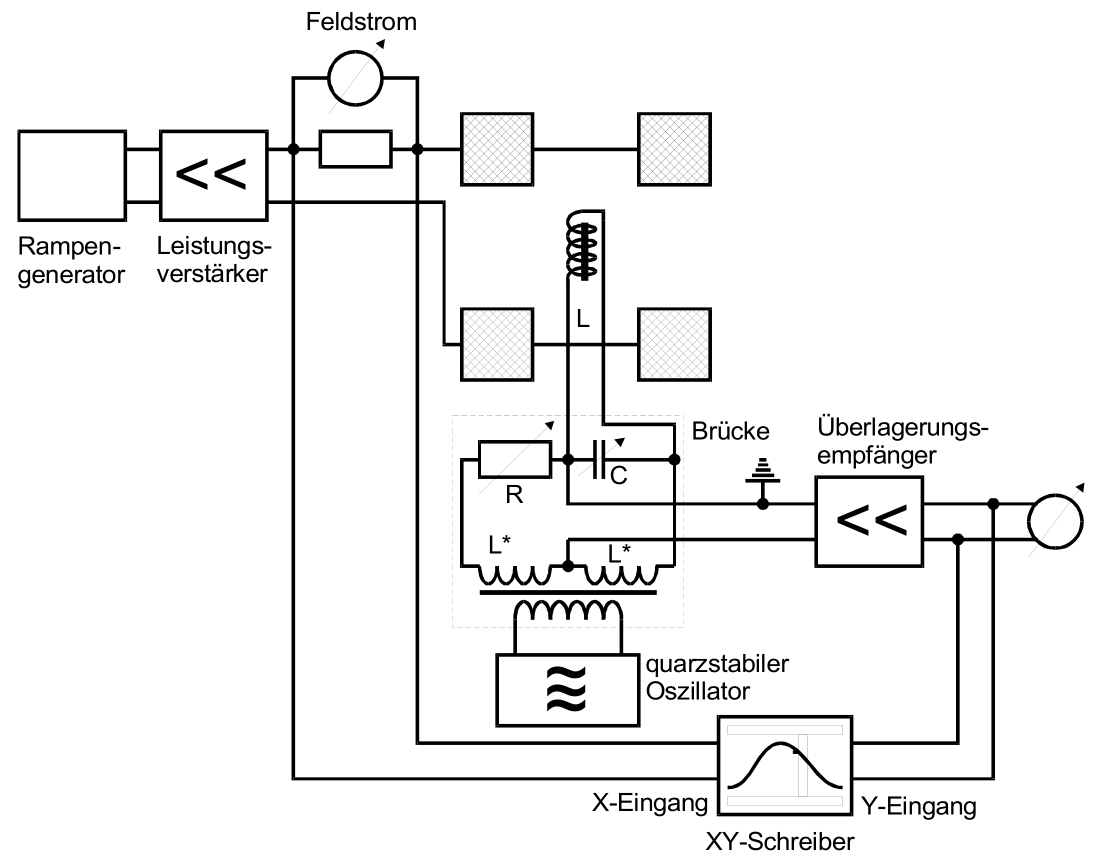
\includegraphics[width=\textwidth]{ESR2.png}
  \caption{Schematische Darstellung der Messapparatur zur ESR \cite{skript}.}
  \label{fig:ESR2}
\end{figure}

Zunächst wird mit Hilfe eines Kompass die Apparatur so ausgerichtet, sodass das Erdmagnetfeld parallel bzw. antiparallel zu den Feldlinien der Helmholtzspule ist.
Als nächstes müssen die Brücke und der Überlagerungsempfänger auf die Frequenz des Vorverstärkers $\nu_e$ abgeglichen werden, da
\begin{equation*}
  \nu_{\text{e}} = \nu_{\text{Osz}} + \nu_{\text{ZF}}
\end{equation*}
gilt.
Dabei ist $\nu_{\text{ZF}}$ die Schwebungsfrequenz von der variablen Messfrequenz $\nu_{\text{e}}$ und der konstant einstellbaren Frequenz des Überlagerungsoszillators $\nu_{\text{Osc}}$.
Nachdem eine Frequenz $\nu_{\text{Osz}}$ eingestellt wurde, wird eine hochfrequente Spannung variiert, bis der Maximalwert der Brückenspannung erreicht wird.
Daraufhin wird die Brücke abgeglichen, indem die Kapazität $C$ und der Widerstand $R$ variiert werden.
Der ZF-Verstärker muss schließlich auf voller Verstärkung eingestellt sein.
Schließlich wird die Brücke wieder mit dem R-Stellglied verstimmt, damit die Resonanzstelle hinterher auf dem XY-Schreiber in Form von einem Maximum oder Minimum abzulesen ist.
Der Vorgang wird wiederholt, indem die Pole der Helmholtzspule getauscht werden, damit hinterher der Einfluss des Erdmagnetfeldes berücksichtigt wird.
